\documentclass[english,man]{apa6}

\usepackage{amssymb,amsmath}
\usepackage{ifxetex,ifluatex}
\usepackage{fixltx2e} % provides \textsubscript
\ifnum 0\ifxetex 1\fi\ifluatex 1\fi=0 % if pdftex
  \usepackage[T1]{fontenc}
  \usepackage[utf8]{inputenc}
\else % if luatex or xelatex
  \ifxetex
    \usepackage{mathspec}
    \usepackage{xltxtra,xunicode}
  \else
    \usepackage{fontspec}
  \fi
  \defaultfontfeatures{Mapping=tex-text,Scale=MatchLowercase}
  \newcommand{\euro}{€}
\fi
% use upquote if available, for straight quotes in verbatim environments
\IfFileExists{upquote.sty}{\usepackage{upquote}}{}
% use microtype if available
\IfFileExists{microtype.sty}{\usepackage{microtype}}{}

% Table formatting
\usepackage{longtable, booktabs}
\usepackage{lscape}
% \usepackage[counterclockwise]{rotating}   % Landscape page setup for large tables
\usepackage{multirow}		% Table styling
\usepackage{tabularx}		% Control Column width
\usepackage[flushleft]{threeparttable}	% Allows for three part tables with a specified notes section
\usepackage{threeparttablex}            % Lets threeparttable work with longtable

% Create new environments so endfloat can handle them
% \newenvironment{ltable}
%   {\begin{landscape}\begin{center}\begin{threeparttable}}
%   {\end{threeparttable}\end{center}\end{landscape}}

\newenvironment{lltable}
  {\begin{landscape}\begin{center}\begin{ThreePartTable}}
  {\end{ThreePartTable}\end{center}\end{landscape}}

  \usepackage{ifthen} % Only add declarations when endfloat package is loaded
  \ifthenelse{\equal{\string man}{\string man}}{%
   \DeclareDelayedFloatFlavor{ThreePartTable}{table} % Make endfloat play with longtable
   % \DeclareDelayedFloatFlavor{ltable}{table} % Make endfloat play with lscape
   \DeclareDelayedFloatFlavor{lltable}{table} % Make endfloat play with lscape & longtable
  }{}%



% The following enables adjusting longtable caption width to table width
% Solution found at http://golatex.de/longtable-mit-caption-so-breit-wie-die-tabelle-t15767.html
\makeatletter
\newcommand\LastLTentrywidth{1em}
\newlength\longtablewidth
\setlength{\longtablewidth}{1in}
\newcommand\getlongtablewidth{%
 \begingroup
  \ifcsname LT@\roman{LT@tables}\endcsname
  \global\longtablewidth=0pt
  \renewcommand\LT@entry[2]{\global\advance\longtablewidth by ##2\relax\gdef\LastLTentrywidth{##2}}%
  \@nameuse{LT@\roman{LT@tables}}%
  \fi
\endgroup}


  \usepackage{graphicx}
  \makeatletter
  \def\maxwidth{\ifdim\Gin@nat@width>\linewidth\linewidth\else\Gin@nat@width\fi}
  \def\maxheight{\ifdim\Gin@nat@height>\textheight\textheight\else\Gin@nat@height\fi}
  \makeatother
  % Scale images if necessary, so that they will not overflow the page
  % margins by default, and it is still possible to overwrite the defaults
  % using explicit options in \includegraphics[width, height, ...]{}
  \setkeys{Gin}{width=\maxwidth,height=\maxheight,keepaspectratio}
\ifxetex
  \usepackage[setpagesize=false, % page size defined by xetex
              unicode=false, % unicode breaks when used with xetex
              xetex]{hyperref}
\else
  \usepackage[unicode=true]{hyperref}
\fi
\hypersetup{breaklinks=true,
            pdfauthor={},
            pdftitle={Bulletproof Bias? Considering the Type of Data in Common Proportion of Variance Effect Sizes},
            colorlinks=true,
            citecolor=blue,
            urlcolor=blue,
            linkcolor=black,
            pdfborder={0 0 0}}
\urlstyle{same}  % don't use monospace font for urls

\setlength{\parindent}{0pt}
%\setlength{\parskip}{0pt plus 0pt minus 0pt}

\setlength{\emergencystretch}{3em}  % prevent overfull lines

\ifxetex
  \usepackage{polyglossia}
  \setmainlanguage{}
\else
  \usepackage[english]{babel}
\fi

% Manuscript styling
\captionsetup{font=singlespacing,justification=justified}
\usepackage{csquotes}
\usepackage{upgreek}



\usepackage{tikz} % Variable definition to generate author note

% fix for \tightlist problem in pandoc 1.14
\providecommand{\tightlist}{%
  \setlength{\itemsep}{0pt}\setlength{\parskip}{0pt}}

% Essential manuscript parts
  \title{Bulletproof Bias? Considering the Type of Data in Common Proportion of
Variance Effect Sizes}

  \shorttitle{Bulletproof Bias?}


  \author{Erin M. Buchanan\textsuperscript{1}~\& John E. Scofield\textsuperscript{2}}

  \def\affdep{{"", ""}}%
  \def\affcity{{"", ""}}%

  \affiliation{
    \vspace{0.5cm}
          \textsuperscript{1} Missouri State University\\
          \textsuperscript{2} University of Missouri  }

  \authornote{
    \newcounter{author}
    Erin M. Buchanan, Department of Psychology, Missouri State University;
    John E. Scofield, Department of Psychological Sciences, University of
    Missouri. Both authors contributed equally to the creation of all parts
    of this manuscript.

                      Correspondence concerning this article should be addressed to Erin M. Buchanan, 901 S National, Springfield, MO, 65897. E-mail: \href{mailto:erinbuchanan@missouristate.edu}{\nolinkurl{erinbuchanan@missouristate.edu}}
                          }


  \abstract{As effect sizes gain ground as important indicators of practical
significance and as a meta-analytic tool, we must critically understand
their limitations and biases. This project investigates the positive
bias of eta squared and critical suggestions of the alternative use of
omega squared or epsilon for their mitigation of bias. Variance overlap
effect sizes were examined for potential bias in different data
scenarios (i.e.~truncated and Likert type data) to elucidate differences
in bias from previous research. We found that data precision and
truncation affected effect size bias, often lowering the bias in eta
squared. This work expands our understanding of bias on variance overlap
measures and allows researchers to make an informed choice about the
type of effect to report given aspects of their research study.
Implications for sample size planning and power are also discussed.}
  \keywords{bias, eta, omega, epsilon \\

    
  }





\usepackage{amsthm}
\newtheorem{theorem}{Theorem}
\newtheorem{lemma}{Lemma}
\theoremstyle{definition}
\newtheorem{definition}{Definition}
\newtheorem{corollary}{Corollary}
\newtheorem{proposition}{Proposition}
\theoremstyle{definition}
\newtheorem{example}{Example}
\theoremstyle{definition}
\newtheorem{exercise}{Exercise}
\theoremstyle{remark}
\newtheorem*{remark}{Remark}
\newtheorem*{solution}{Solution}
\begin{document}

\maketitle

\setcounter{secnumdepth}{0}



\subsection{Null Hypothesis Significance
Testing}\label{null-hypothesis-significance-testing}

Null hypothesis significance testing (NHST) has dominated the social
sciences for the past century, and currently, a blend of the Fisher and
Neyman-Pearson methods are taught and practiced in psychological
research (Gigerenzer, 2004). However, the sole use of NHST can be
inadequate in terms of statistical inference (Kirk, 2003). Statistical
reform is slow, hindering growth in the use of effect sizes (A. Fritz,
Scherndl, \& Kuhberger, 2013; C. O. Fritz, Morris, \& Richler, 2012),
confidence intervals, or even error bars on graphs (Cumming \& Finch,
2005; Cumming et al., 2007). While a detailed discussion of the
criticisms of NHST is outside the scope of this article (Kruschke, 2010;
Loftus, 1996; Wagenmakers, 2007), we briefly discuss a few key issues to
highlight the necessity of alternative means of estimation, namely
effect sizes and their confidence intervals. The assumption of the truth
of null hypotheses is erroneous, as they can be falsified with large
enough sample sizes (Cohen, 1990; Tukey, 1991). Two comparisons in the
real world are always, to some degree, different. A continual increase
in sample size will eventually lead to the rejection of the null
hypothesis. As Cohen (1990) says, \enquote{if the null hypothesis is
always false, what's the big deal about rejecting it?} (pg. 1308).

As Kirk (2003) describes, the use of NHST does not actually provide
answers to the pivotal questions surrounding researchers today. NHST
tells us the probability of obtaining observed, or more extreme data,
assuming that the null hypothesis is true (Kruschke, 2011). NHST does
not expound on the probability of a research hypothesis being correct,
begetting a series of misinformed reject-this to accept-that type of
reasoning for supporting research hypotheses. Another criticism of NHST
lies with the encouragement of a dichotomous decision-making paradigm
(i.e.~reject, do not reject). \emph{p}-values, a central component of
dichotomous decision-making, are defined as the probability that data is
equal to, or more extreme than its observed value, given the null
hypothesis is true (Cohen, 1990; Wagenmakers, 2007). However,
\emph{p}-values are often misunderstood and misused (Cumming, 2014;
Gigerenzer, 2004). \emph{p}-values are sometimes assumed to indicate of
the size or strength of an effect (i.e., suggesting that \emph{p}
\textless{} .001 is \emph{very} significant), and questionable research
practices, such as \emph{p}-hacking (Simmons, Nelson, \& Simonsohn,
2011) can lead to artificially significant results and Type I errors.
Effects are dichotomized into significant and non-significant, without
shedding light on the practical importance of findings. Parametric NHST
is also sensitive to the violations of statistical assumptions, given
the common occurrence of non-normal data in some phenomena (Tabachnick
\& Fidell, 2012). Even with recent suggestions to move the \(\alpha\)
criterion to a lower threshold, such as \emph{p} \textless{} .005
(Benjamin et al., 2017), this shift does not ultimately solve inherent
problems with \emph{p}-values and misguided interpretations. Research
hypotheses should not be merely centered on dichotomous decision
criteria and \emph{p}-values, but should consider the magnitude, or
practical significance, of scientific phenomena (Kirk, 2003; Thompson,
2007).

\subsection{Effect Size}\label{effect-size}

Effect sizes are argued to be as, or more, important indicators of
statistical inference than the sole reliance on NHST (Cumming, 2014;
Rosenthal \& Rubin, 1994). Lakens (2013) describes effect sizes as
\enquote{the most important outcome of empirical studies} (pg. 1).
Effect sizes add the ability to interpret the practical importance of a
phenomenon, centered in the context of the research field, alongside or
in place of statistical significance (Cohen, 1994). Additionally, effect
sizes are integral to meta-analyses and \emph{a priori} power analysis
planning. Even though Wilkinson (1999) and the newest style guide
manuals have heavily suggested the use of effect sizes, C. O. Fritz et
al. (2012) and A. Fritz et al. (2013) have shown that report rates of
effect sizes are still low. The current literature shows a renewed
interest in effect sizes, as Google Scholar searches indicate a slew of
publications on effect size and meta-analysis in recent years. While
effect sizes have been suggested as an integral tool of statistical
inference, specific characteristics of multiple effect sizes are still
under scrutiny, with Kirk (2003) noting the development of more than
seventy separate effect size indices.

The majority of effect size estimates can be binned into two families.
The \emph{d} family is generally based on mean differences, whereas the
\emph{r} family is based on the association strength of proportion of
variance explained by manipulated factors (K. Kelley \& Preacher, 2012;
Maxwell \& Delaney, 2004). This article will focus on proportion of
variance effect sizes, specifically, as previous research on the
distribution of the \emph{d} family has inspired this work (Cumming,
2014; Smithson, 2001). Eta squared (\(\eta^2\)), a proportion of
variance effect size, is the most common effect size reported alongside
ANOVAs, even though \(R^2\) utilizes the same formula (Grissom \& Kim,
2005; Matsumoto, Kim, \& Grissom, 2011). \(\eta^2\) is calculated from
the sum of squares associated with the effect and the sum of squares
associated with the error term in a sample, which is interpreted as a
point-estimate for the population (Cumming, 2014; Pearson, 1905).

Effect sizes, however, are not all created equally, as sample-based
effect sizes can overestimate population effects. Maxwell and Delaney
(2004) describe this bias as the likelihood of sample means inevitably
deviating from population means, due to sampling variability. The
positive bias of \(\eta^2\) has been widely recognized, due to its
reliance with least-squares methods associated with \emph{t}-tests and
ANOVA designs, as well as with sampling error variability across
different studies (Shieh, 2008; Skidmore \& Thompson, 2011, 2012; Snyder
\& Lawson, 1993; Stevens, 1992; Thompson, 2006, 2007; Yin \& Fan, 2001).
Multiple bias-correcting formulas have been established to help
\enquote{shrink}, or adjust, the bias from the population and sample
effect size estimates (Olkin \& Pratt, 1958; Raju, Bilgic, Edwards, \&
Fleer, 1999; Stuart, Ord, \& Arnold, 1994), and Yin and Fan (2001)
provide detailed discussion of these formulas and their implementation.
Bias-correcting formulas developed for \(\eta^2\) are not examined
further here because these formulas correct for a general assumption of
positive bias, whereas positive bias was a central question to our
current investigation.

Epsilon squared (\(\epsilon^2\)) was proposed by T. L. Kelley (1935),
offering an alternative, less biased effect size measure. \(\epsilon^2\)
adjusts for positive bias by correcting the numerator in the formula of
\(\eta^2\). This correction occurs by subtracting the mean square error
from the sum of squares treatment (Olejnik \& Algina, 2000). Omega
squared (\(\omega^2\)), introduced by Hays (1963), takes this adjustment
a step further, by not only subtracting the mean square error in the
numerator, but subtracting the mean square error from the sum of squares
total in the denominator as well (Olejnik \& Algina, 2000). Carroll and
Nordholm (1975), however, noted that \(\epsilon^2\) and \(\omega^2\)
yield similar ranges of effect sizes. While the use of \(\omega^2\) and
\(\epsilon^2\) can reduce sampling variability evident in \(\eta^2\),
some have argued that these effect size adjustments do not eliminate
bias entirely (Keselman, 1975; Maxwell \& Delaney, 2004; Okada, 2013,
2017; Olejnik \& Algina, 2000). Maxwell and Delaney (2004) note that
typical differences between \(\omega^2\) and \(\eta^2\) estimates fall
within .02 of each other, while O'Grady (1982) argued that \(\omega^2\)
may also occasionally lead to an underestimation of population effect
size estimates.

\(\omega^2\), like every other effect size estimate, is not without its
limitations. First, \(\omega^2\) may be computationally difficult to
calculate, especially in complex designs, and even textbooks that
discuss \(\omega^2\) detail this limitation (A. Field, Miles, \& Field,
2012). For meta-analytic purposes, \(\omega^2\) generally cannot be
computed because of reliance on sum of squares and mean squared error
values, which have no translatable estimate formula from the
\emph{F}-statistic like \(\eta^2\). Using \(\omega^2\) may be
inappropriate in designs where sample sizes across groups are unequal,
as the model in which \(\omega^2\) was derived assumes a balanced design
(Olejnik \& Algina, 2000; Vaughan \& Corballis, 1969). However, Carroll
and Nordholm (1975) noted that \(\omega^2\) estimations with unequal
\emph{n} negligibly affected estimates, unless combined with
heterogeneous variances.

\subsection{Overall Limitations and
Bias}\label{overall-limitations-and-bias}

Each effect size includes aspects in regards to its use in scientific
research, as well as limitations in its interpretation. This paper
focuses on the bias, standard deviation, and standard error of each
effect to expand on previous research by Okada (2013). Fern and Monroe
(1996) outlined that proportion of variance effect sizes should be
interpreted depending on the type of research design used, whether
treatments were manipulated between- or within-subjects, and whether
experiments contained more than one factor. Researchers should consider
elements, such as measurement reliability, heterogeneity of variance,
the range of treatment manipulations, and the type of scale used before
assigning a value of importance to a given effect size estimate. Large
sample sizes increase accuracy of effect size estimation, as smaller
sample sizes are associated with larger standard errors. This limitation
is especially prevalent with the combination of small sample sizes and
heterogeneous variances (Carroll \& Nordholm, 1975). Others have
commented that sample-based estimates have higher sampling errors with
small \emph{n} (Maxwell \& Delaney, 2004; Thompson, 2007), and that
differences in effect sizes, such as \(\eta^2\), \(\omega^2\), and
\(\epsilon^2\), tend to converge as sample size substantially increases
(Maxwell, Camp, \& Arvey, 1981).

Several previous studies have examined the interplay between bias,
standard deviation, and standard error, mostly focusing on sample size
and effect size as variables of interest. Keselman (1975) ran 1,000
simulations of ANOVAs and determined that \(\omega^2\) estimates were
closer to the population effect than both \(\epsilon^2\) and \(\eta^2\).
\(\omega^2\) has been advocated as the \enquote{nearly unbiased}
estimator of the population effect, wherein \(\omega^2\) has less bias
than \(\epsilon^2\), leaving \(\eta^2\) as the most biased (Grissom \&
Kim, 2005; Matsumoto et al., 2011). However, \(\omega^2\) can be
negatively (i.e.~underestimate) biased, as originally found in Carroll
and Nordholm (1975) and replicated in O'Grady (1982). Okada (2013)
extended these results by comparing all three effect sizes across sample
size and mean variability by simulating 1,000,000 one-way fixed effect
ANOVAs with four treatment levels. While Okada used 1,000,000
simulations, many researchers have concluded that far fewer simulations
can achieve an adequate attenuation of sampling variability (Fan,
Felsovalyi, Sivo, \& Keenan, 2001; Robey \& Barcikowski, 1992; Skidmore
\& Thompson, 2012).

Results from Okada (2013) revealed that, \(\epsilon^2\), not
\(\omega^2\), held the least bias across \emph{n}. \(\omega^2\) did,
however, outperform both \(\epsilon^2\) and \(\eta^2\) in standard
error. \(\eta^2\) did have the lowest standard deviation, but Okada
notes that \(\eta^2\) performed poorly considering both bias and
standard error. Okada concluded with a firm cautionary warning that
researchers should not use \(\eta^2\), as it incorrectly overestimates
the population effect across sample, inversely related to sample size.
Skidmore and Thompson (2012) also investigated the performance of these
effect sizes, considering common statistical assumption violations like
heterogeneity, and found similar results as previous simulation studies
(Carroll \& Nordholm, 1975; Keselman, 1975; Okada, 2013). Even though
these studies have focused on slightly different facets of bias in
one-way between-subjects ANOVA, a common theme has emerged. Even with
bias decreasing as an additive function of both an increase in
population effect size and sample size (Maxwell \& Delaney, 2004),
conclusions from these studies remain the same: \(\eta^2\) should not be
used. This conclusion is intriguing, largely because \(\eta^2\) is
readily presented among statistical software packages (e.g.~SPSS, R,
JASP) and continues to be the most commonly reported effect size for
ANOVA type designs (Lakens, 2013).

\subsection{Purpose of Current Study}\label{purpose-of-current-study}

The purpose of the current study is to examine these important
conclusions regarding the use of \(\eta^2\), as well as examining the
type of data used in research design and its effects on the performance
of \(\eta^2\), \(\epsilon^2\), and \(\omega^2\). While former studies
have investigated cases when ANOVA model assumptions hold true, we
investigated the case when aspects do not hold true, which is often
reflected in cases of real psychological data analysis.

We first established empirical confidence intervals of bias, standard
deviation, and standard error to use as a criterion for judging changes
in these variables. Second, we examined the effect of data type on bias,
standard deviation, and standard error. Last, for the data type
manipulations that significantly change bias, standard deviation, or
standard error, we calculated this change across a large range of effect
sizes (i.e.~nearly zero to very large). This analysis demonstrates the
effect of the bias, standard deviation, or standard error change with
more precision than previous work binning effect sizes into small,
medium, or large magnitudes.

\section{Method}\label{method}

\subsection{Simulations}\label{simulations}

To further the work by Okada (2013), it is first advantageous to explain
the underlying assumptions and formulas used in this extension. While
these formulas can be found in many introductory statistics textbooks
covering ANOVA methods, we describe them below as well as provide
\emph{R} syntax online to aid in the reproducibility and understanding
of the current extension. Population effect size is calculated by
creating a sum of squares for between group differences from the grand
mean:

\[
SS_{between} = \frac{\Sigma (\bar{X_{i}} - \bar{X})^2} {N_{groups}}
\] and then determining group error with an average of group variances.
In this formula, \(\bar{X_{i}}\) indicates each proposed group mean,
while \(\bar{X}\) is the proposed grand average of group means.
Population eta is then calculated by creating a ratio of
\(SS_{between}\) and \(SS_{error}\), analogous to the full \(\eta^2\)
formula:

\[
\eta^2_{pop} = \frac{SS_{between}} {SS_{between} + SS_{error}}.
\] \(SS_{error}\) is calculated by averaging all proposed group
variances. Specifically, we used standard deviations of one to match
previous simulations, but this point for calculation of \(\eta^2_{pop}\)
from \emph{R} syntax should be clarified for interested parties (i.e.,
the previous syntax included a value of one, while this value is
calculated from group variances and should not be a set number). The
value of one in the denominator is an expected average of group
variances, which is approximately one in these examples. This value
should be changed for simulations with heterogeneity or other proposed
standard deviations.

Bias is estimated by calculating the average simulated \(\eta^2\) values
and subtracting the \(\eta^2_{pop}\) estimate. This value represents the
effect size deviation from the population, wherein positive numbers
represent an inflation of effect size due to manipulated variables,
while negative numbers indicate a reduction in effect size estimates,
compared to population values. Standard deviation (SD) and root mean
squared error (standard error; RMSE) of the effect size are simple
adjustments of the traditional standard deviation formula:

\[
SD = \sqrt\frac{\Sigma (\eta^2_{i} - \bar{\eta^2})^2} {N_{sims}}
\] and:

\[
RMSE = \sqrt\frac{\Sigma (\eta^2_{i} - \eta^2_{pop})^2} {N_{sims}}.
\] Here, sample SD is calculated by squaring the difference between the
estimated \(\eta^2_{i}\) for each simulation from the mean
\(\bar{\eta^2}\) of that sample size. RMSE estimates the standard error
by squaring the differences of estimated \(\eta^2_{i}\) for each
simulation from the \(\eta^2_{pop}\). Both formulas use the population
sample size estimator (\(N_{sims}\)) in the denominator, rather than
degrees of freedom (i.e., \(N_{sims}\) - 1). This formula is consistent
with previous work by Okada (2013) and is appropriate for simulation
studies (i.e., with large simulation numbers, results are consisent with
\emph{N} or \emph{N}-1).

\subsection{Manipulated Variables}\label{manipulated-variables}

Using the cited simulation code, we manipulated several factors
independently to determine the effects of data type on bias, SD, and
RMSE of variance overlap effect sizes. Methodologically, we examined the
number of simulations first in \emph{R}. For data types, we varied the
number of decimals, type of means, and truncation/skew of the data. In
all simulations testing these variables, we used the largest variability
condition from Okada (2013) (i.e.~means 0.0, 0.0, 1.2, 1.2) because it
showed the largest bias, SD, and RMSE effects. Each simulation was
tested across sample size values and effect size types found in Okada
(2013). The \emph{R} code from our study can be found at
\url{http://osf.io/urd8q} in an \emph{R} markdown file that shows the
simulation and graph code inline with this manuscript.

\section{Results}\label{results}

\subsection{Confidence Intervals}\label{confidence-intervals}

1,000 simulations per condition was used for this study. This option can
be practical for researchers in terms of computation time, as results
using 1,000 simulations are remarkably similar to Okada (2013). From one
hundred iterations of 1,000 simulations, empirical 95\% confidence
intervals were calculated by taking the 2.5\% and 97.5\% values
(i.e.~values ranked 2 and 3 were averaged or values 97 and 98 were
averaged). Confidence intervals are very small around average scores,
indicating a reasonable range of values to be found. Graphs depicting
this finding can be found online at \url{http://osf.io/urd8q}. The
empirical confidence interval calculated here was used to determine how
bias, SD, and RMSE changed across data type manipulations.

\subsection{Precision of the Dependent
Variable}\label{precision-of-the-dependent-variable}

We also explored the effect of the type of dependent variable on bias,
RMSE, and SD, starting with the precision of the dependent variable.
\emph{rnorm()} calculates random numbers to 16 decimal places. With
computer assisted data collection, some phenomena may be calculated with
more precision (i.e.~more decimals), but it is unlikely that all data is
collected with a large number of significant digits. Additionally, if
researchers use Likert type data, it is possible that dependent
variables may be captured in whole numbers. We simulated 1,000 datasets
and within each round, we calculated bias, RMSE, and SD on the same
data, rounding values from 0 to 15 decimals. After examining these data,
only very small changes were apparent through one decimal (i.e.~1-15
decimals do not show differences larger than .001), and therefore, we
only present results from rounding to the least precision, zero
decimals. The complete dataset and code for both of these simulations
are presented online at \url{http://osf.io/urd8q}.

\begin{figure}
\centering
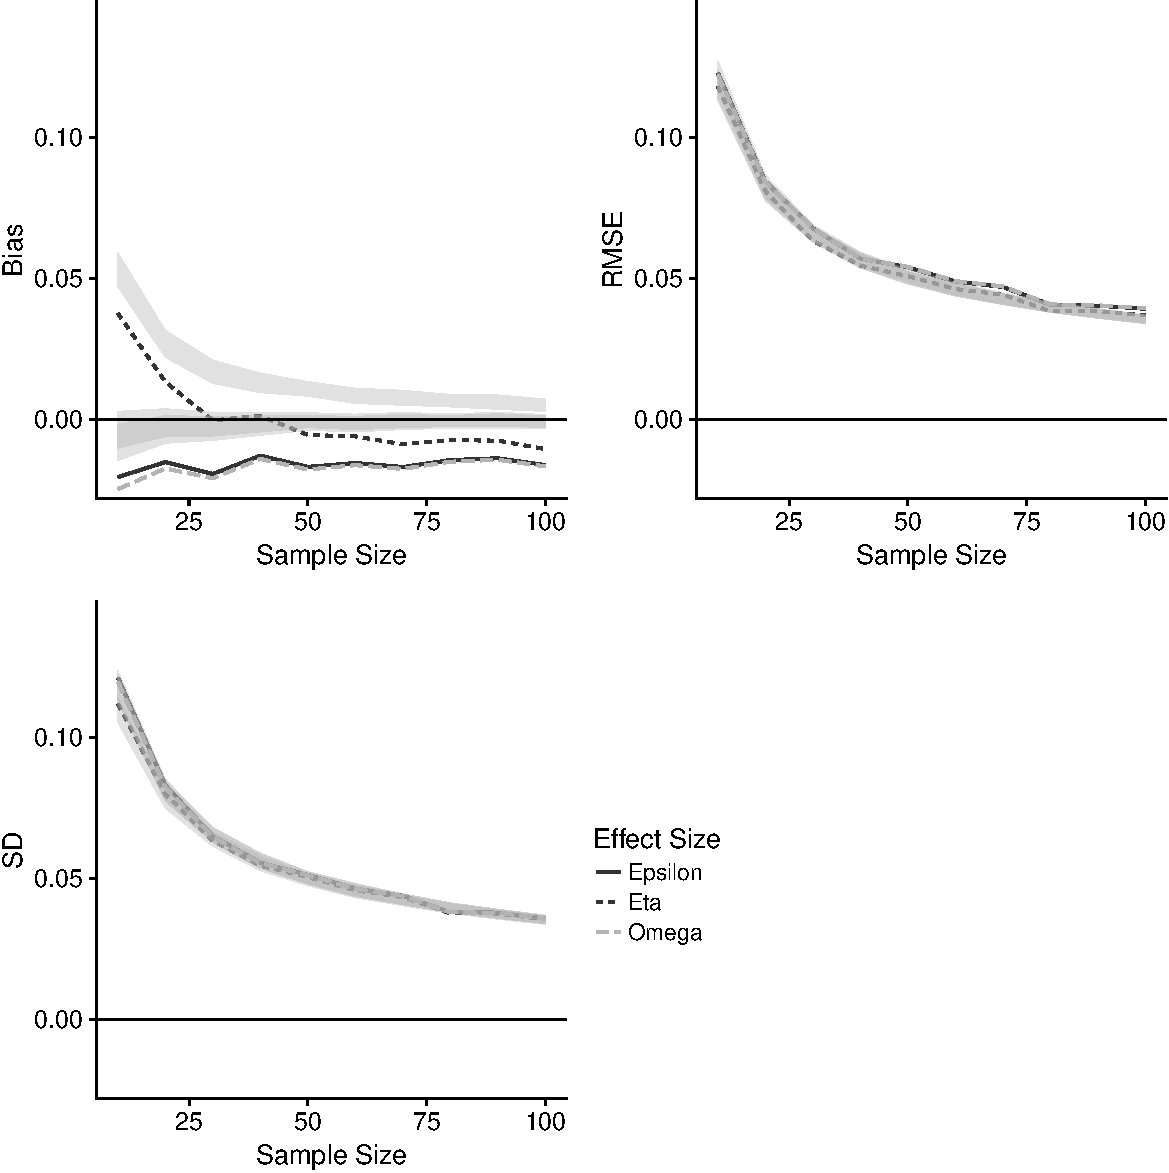
\includegraphics{buchanan_scofield_version2_files/figure-latex/decimal-graph-1.pdf}
\caption{\label{fig:decimal-graph}Bias, SD, and RMSE values of zero decimal
dependent variables. Shaded gray area represents 95\% confidence
interval around these values.}
\end{figure}

As seen in Figure \ref{fig:decimal-graph}, rounding the dependent
variable to zero decimals had a stark effect on the bias found in each
of the effect sizes. All three were downwardly affected, that is, using
less precise dependent variables resulted in less upwardly biased effect
sizes. In fact, both \(\omega^2\) and \(\epsilon^2\) were completely
negatively biased, and \(\eta^2\) showed a negative bias after sample
sizes approximately \emph{n} = 40. These values average 0.012 outside
the comparison CI created in the first stage of this paper, which is
traditionally considered a small effect size for variance overlap
measures (Cohen, 1992). RMSE values were increased outside the
confidence interval for \(\omega^2\) and \(\epsilon^2\) across most
\emph{n} values over 50, averaging 0.002 over the comparison CI.
However, the SD for each effect size was unaffected by the rounding to
whole numbers. Interested readers can view an interactive Shiny
application on our OSF page. The Shiny app allows users to view figures
in color, as well as manipulate the y-axis. Precise decimals are
included with each figure, and while we report RMSE values here outside
the CI created to examine changes, a reader can interpret these values
with their own criteria online. With these results, we do not suggest
that researchers should use less precise dependent variables; however,
it is important to consider that effect size estimates from rounded data
may be under-representing the size of their population effects and a bit
more variable than expected.

\subsection{Type of Dependent Variable and Data
Skew}\label{type-of-dependent-variable-and-data-skew}

Given that Likert data is generally represented as whole numbers, we
examined the effect of Likert type dependent variables may indirectly
change effect sizes. Often, Likert scales are criticized for their
non-normal distributions (Bishop \& Herron, 2015), where participants
will choose only the ends of the scale. Therefore, in this set of
simulations we first examined the effect of simply shifting the
estimated sample means over to 2, 2, 3.2, and 3.2 to mimic a floor
effect on a traditional 1-7 style scale. 1,000 simulations indicated no
large differences from the comparison study (part one of this paper),
and therefore, all data and graphs are presented online for the
interested reader. After confirming that we did not see changes by
shifting away from a standard normal distribution, we then simulated
1,000 datasets with adjusted means that were truncated. This procedure
rounded all values less than one to one, and all values over seven down
to seven. In each of these simulation tests, we only manipulated one
variable, and therefore, the data in this test were otherwise not
rounded (i.e.~precision was set to default decimals).

\begin{figure}
\centering
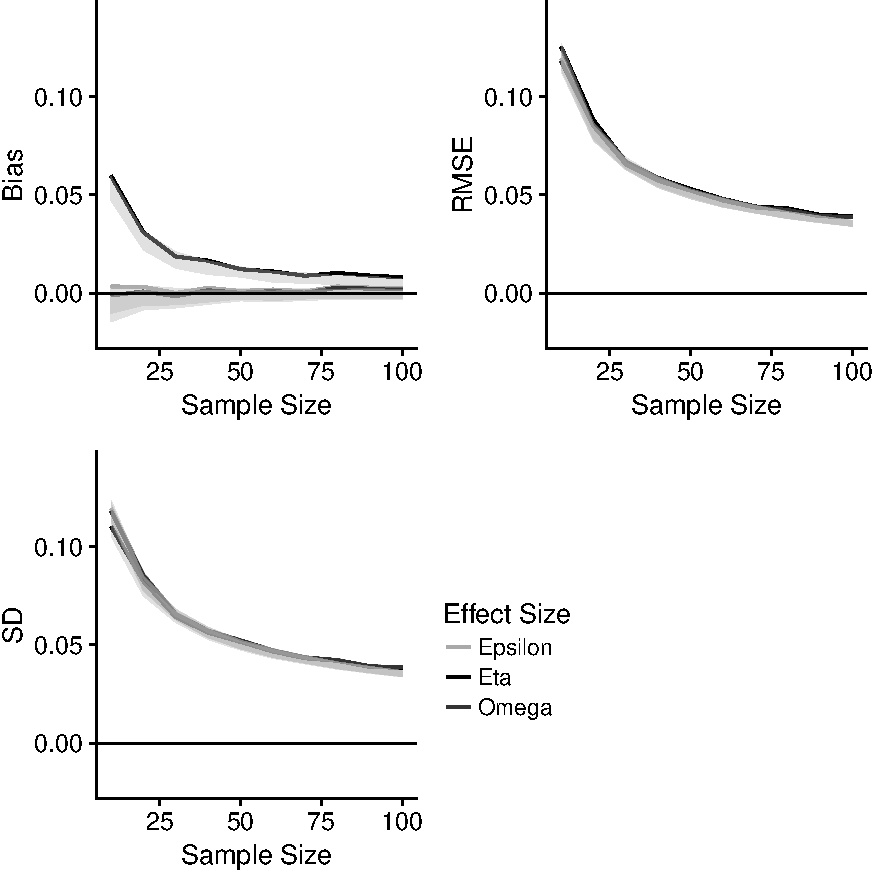
\includegraphics{buchanan_scofield_version2_files/figure-latex/likerttrun-graph-1.pdf}
\caption{\label{fig:likerttrun-graph}Bias, SD, and RMSE values for truncated
Likert style dependent variables. Shaded gray area represents 95\%
confidence interval around these values.}
\end{figure}

This simulation set showed the opposite effect of rounding, namely that
bias was increased with truncated data, especially at low \emph{n} (10)
and upper \emph{n} (above 60), with an average of 0.001 increase outside
the confidence interval. RMSE and SD were similarly increased 0.001 for
all effect sizes at both low (\emph{n} = 20) and high (\emph{n} = 80+)
ends. Figure \ref{fig:likerttrun-graph} includes the graphs of these
results.

\subsection{Changes Across Effect
Size}\label{changes-across-effect-size}

In summary, our simulations showed that several aspects of the data
change the bias and variance of effect sizes compared to a population
parameter. These simulations were calculated on the largest effect from
the Okada (2013) to show the greatest possible differences, and the
population effect size was set to .265. In this section, we expand the
original research and our findings to a range of effect sizes. The
simulation code was modified to start with a very small effect size,
.012, and increase to a very large effect size, .679. We achieved this
range by creating a mean vector that started with zero and each
subsequent mean was increased by a decimal additive. This decimal
additive started at 0.10 and increased to 1.30 in 0.05 increments.
Therefore, the first mean vector was (0, 0.1, 0.2, 0.3) and the last
mean vector was (0.0, 1.3, 2.6, 3.9). This procedure increased the
population effect size estimate approximately .02 to .04 at a time. The
upper end of the range of possible effect sizes estimated was chosen so
that the effects of Likert truncation could be examined by starting
means at 2.0 and staying within a range of 1-7.

\begin{figure}
\centering
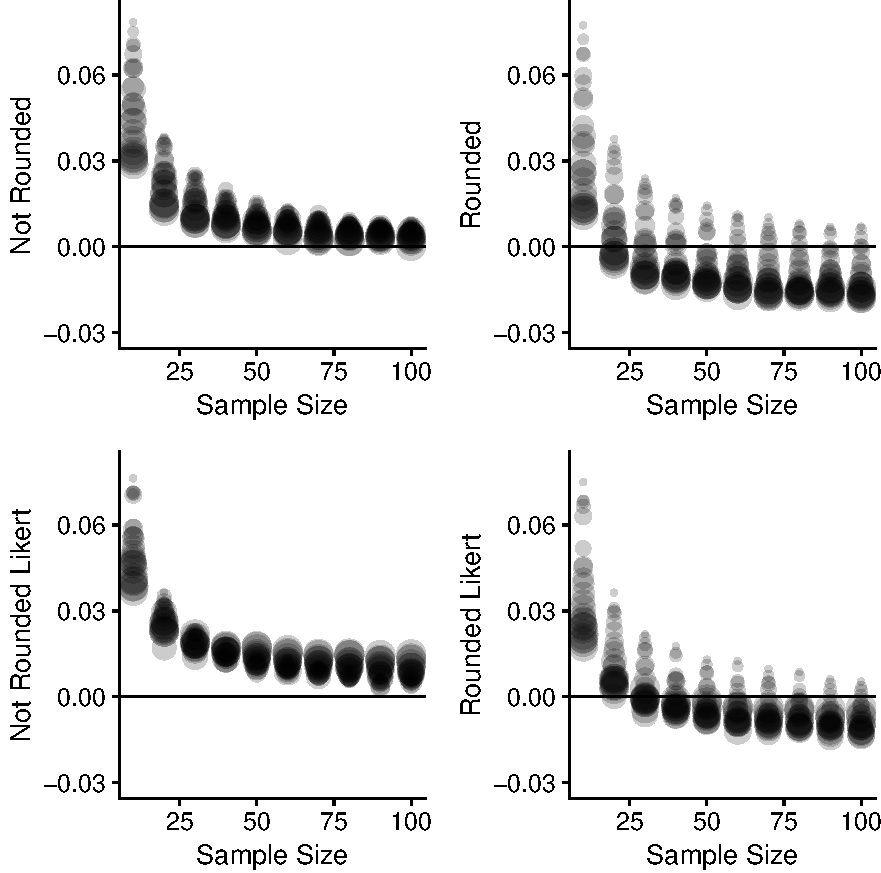
\includegraphics{buchanan_scofield_version2_files/figure-latex/across-graph-bias-1.pdf}
\caption{\label{fig:across-graph-bias}Bias values for eta squared for
regular and truncated Likert data (top and bottom) that has been not
been rounded or rounded to whole numbers (left and right). Circle size
indicates population eta squared values, wherein small dots are small
effect sizes and large dots are large effect sizes.}
\end{figure}

\begin{figure}
\centering
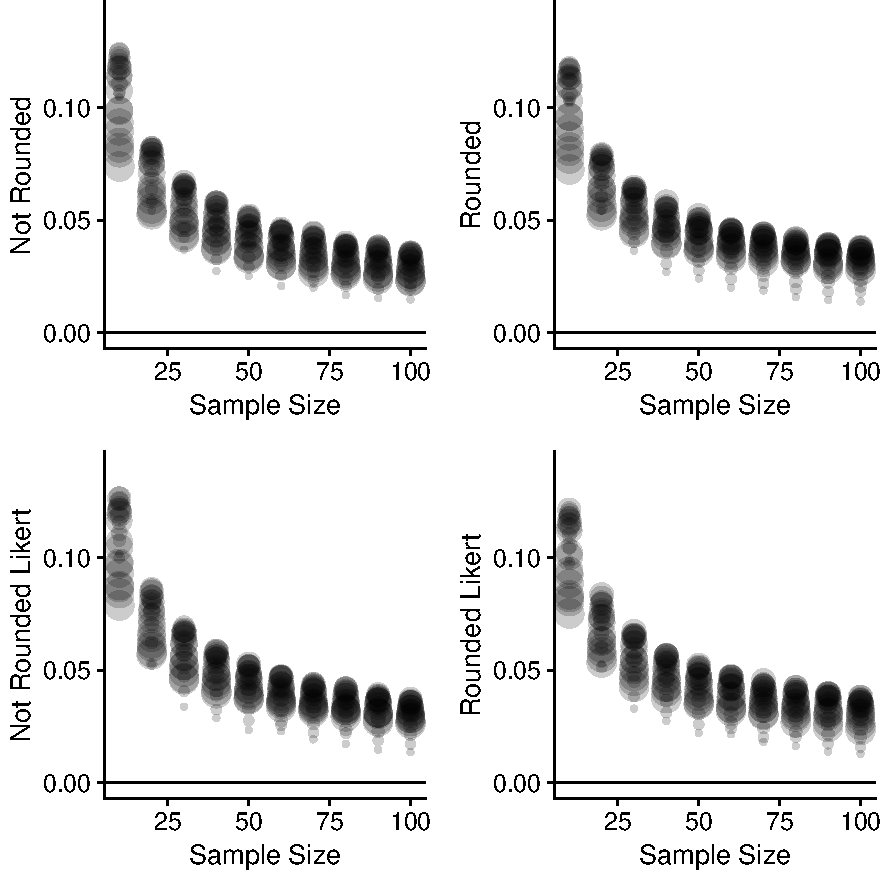
\includegraphics{buchanan_scofield_version2_files/figure-latex/across-graph-rmse-1.pdf}
\caption{\label{fig:across-graph-rmse}RMSE values for eta squared for
regular and truncated Likert data (top and bottom) that has been not
been rounded or rounded to whole numbers (left and right). Circle size
indicates population eta squared values, wherein small dots are small
effect sizes and large dots are large effect sizes.}
\end{figure}

\begin{figure}
\centering
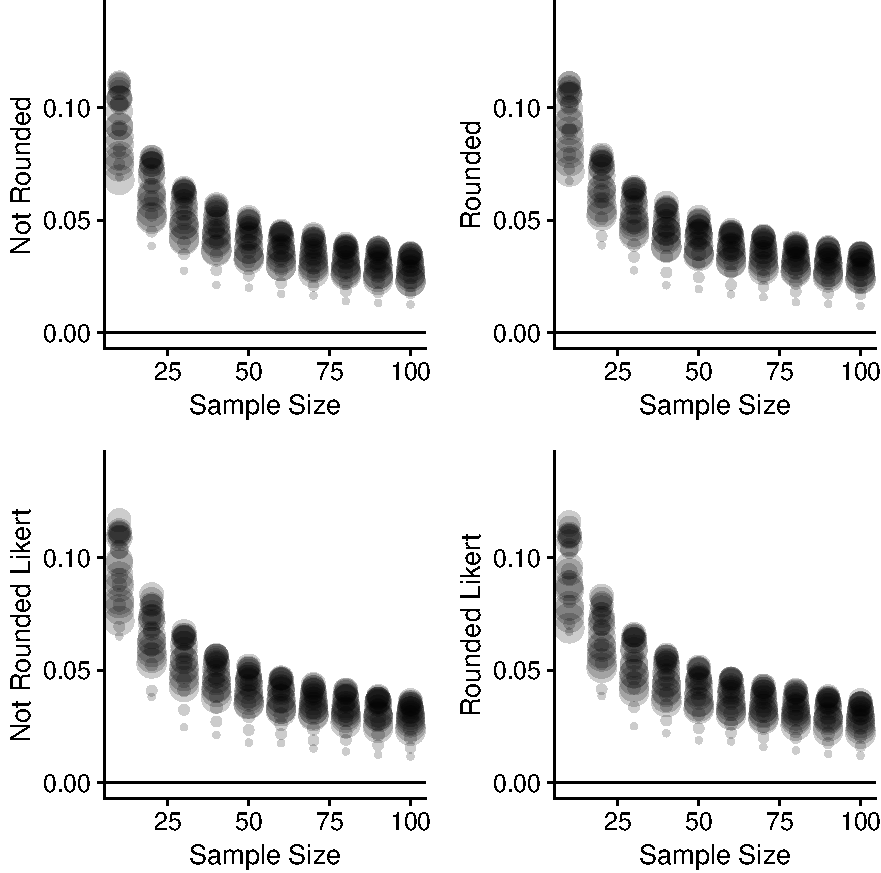
\includegraphics{buchanan_scofield_version2_files/figure-latex/across-graph-sd-1.pdf}
\caption{\label{fig:across-graph-sd}SD values for eta squared for regular
and truncated Likert data (top and bottom) that has been not been
rounded or rounded to whole numbers (left and right). Circle size
indicates population eta squared values, wherein small dots are small
effect sizes and large dots are large effect sizes.}
\end{figure}

Because of the complexity of this data, only \(\eta^2\) values were
plotted to show the effect of rounding and truncation across a large
range of effect sizes. \(\eta^2\) was chosen as it is the most commonly
reported effect size for ANOVA type designs (Lakens, 2013). Effects of
rounding and truncation are similar across different effect size types,
and interested readers can change code in Rmarkdown document to view
\(\omega^2\) and \(\epsilon^2\). Figure \ref{fig:across-graph-bias}
indicates the bias of \(\eta^2\), and the effect of rounding was wider
spread across the range of sample size, while non-rounded data converges
across sample size. Truncated Likert data showed a similar pattern with
slightly less spread than regular data, as well as a slight upward
increase in bias, as shown above. Figure \ref{fig:across-graph-rmse}
portrays the subtle effect of rounding and truncation increasing values
at the low and high ends of sample size. A new finding shown here was
that RMSE appears to be lowest at low and high population effect sizes
peaking at \(M_{NZ}\) = 0.27, \(M_{RZ}\) = 0.32, \(M_{NL}\) = 0.28, and
\(M_{RL}\) = 0.35 (with the subscript N for not rounded data, R for
rounded data, Z for normal data, and L for truncated Likert data). SD
calculation shown in Figure \ref{fig:across-graph-sd} displays the same
pattern with similar average peak values: \(M_{NZ}\) = 0.29, \(M_{RZ}\)
= 0.32, \(M_{NL}\) = 0.33, and \(M_{RL}\) = 0.29.

\subsection{Sample Size Planning}\label{sample-size-planning}

\begin{figure}
\centering
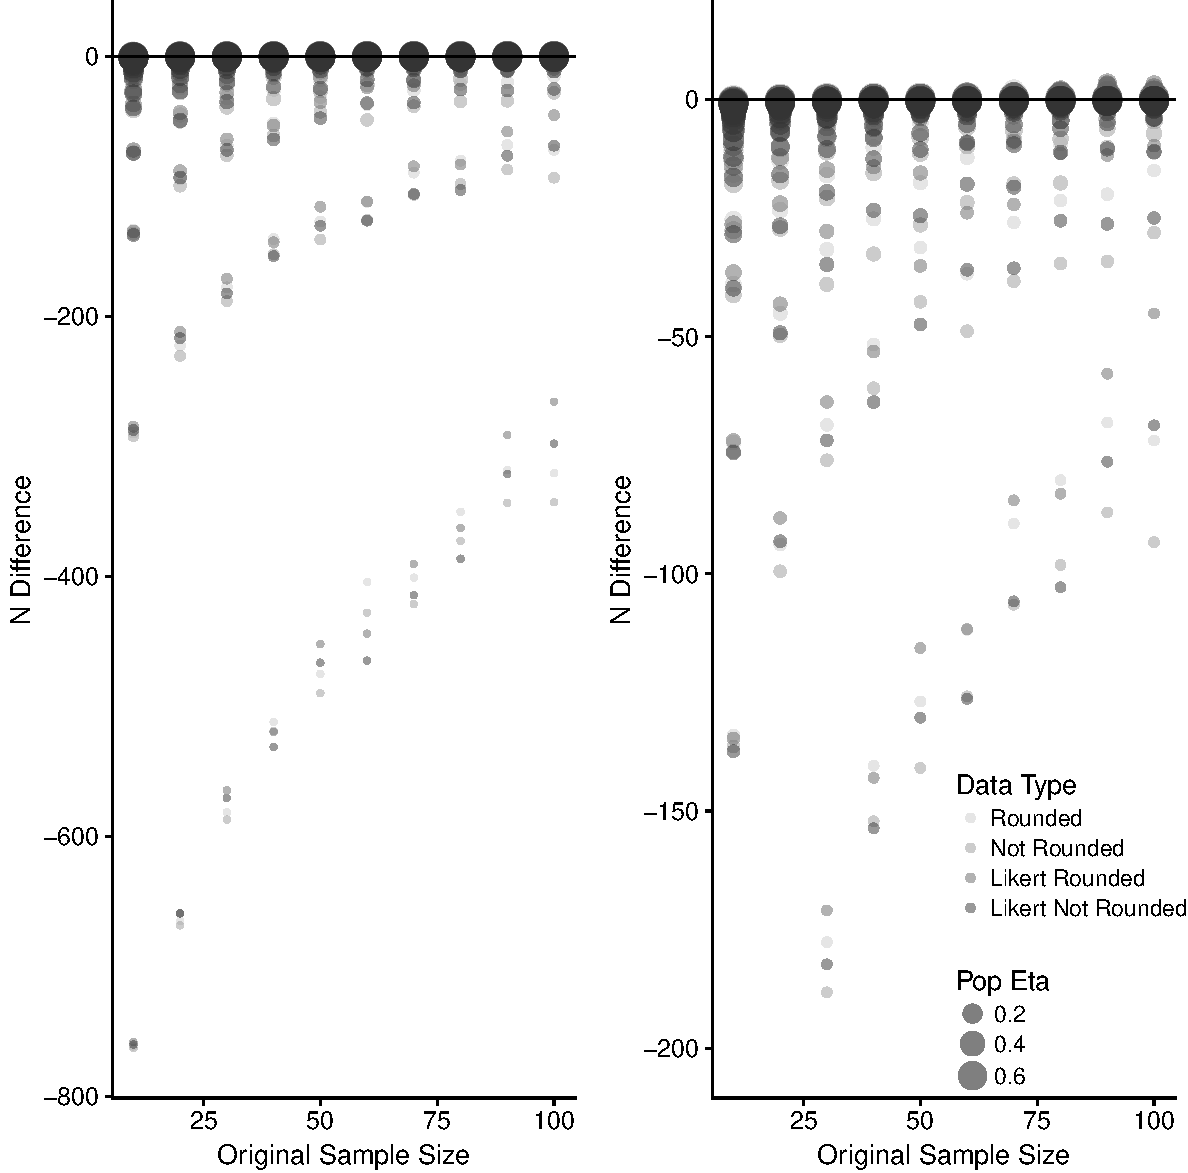
\includegraphics{buchanan_scofield_version2_files/figure-latex/powerL-graph-1.pdf}
\caption{\label{fig:powerL-graph}Sample size differences estimated for 80\%
power for found versus population effect sizes. Negative values indicate
an underestimation of sample size needed to detect a significant effect.
Circle size indicates population eta squared values, wherein small dots
are small effect sizes and large dots are large effect sizes. The left
panel indicates the full range of the data, while the right panel is
zoomed in to show the effects at larger population values.}
\end{figure}

This research primarily focused on the effects of changing dependent
variables on bias estimates for variance overlap effect sizes.
Generally, \(\eta^2\) is biased at smaller sample sizes and less biased
at larger effect sizes, while \(\omega^2\) and \(\epsilon^2\) are
generally slightly negatively biased. The type of dependent data,
rounded and truncated, can decrease or increase that bias. These values
become practically important for sample size planning for future
studies. Therefore, we calculated the sample size necessary to attain
80\% power with an \(\alpha\) of .05 using the \emph{pwr} library
(Champely, 2016) for both the population and observed \(\eta^2\) values
for the data calculated in the last section. We focused on \(\eta^2\)
because of its popularity among researchers, and the differences in bias
were apparent across sample size. Figure \ref{fig:powerL-graph}
indicates the proposed sample size difference between population and
observed \(\eta^2\) across original sample size. The left panel includes
the full range of population \(\eta^2\), while the right panel zooms in
to larger population \(\eta^2\) values. All four data types (rounded
versus not, Likert versus not) are included in different gray shades,
but these estimates are very similar, especially around zero sample size
differences. The main takeaway from this graph is the extreme
underestimation of suggested sample size at small effect sizes, as they
are often the most biased (see Figure \ref{fig:across-graph-bias}). The
average underestimation was close to 30 participants for each type of
dependent variable: \(M_{NZ}\) = -32.60, \emph{SD} = 106.26; \(M_{RZ}\)
= -29.25, \emph{SD} = 103.95; \(M_{NL}\) = -31.86, \emph{SD} = 105.01;
\(M_{RL}\) = -28.29, \emph{SD} = 102.60. The minimum values (largest
underestimation) were large for small population effect sizes: \emph{NZ}
= -762.95; \emph{RZ} = -761.54; \emph{NL} = -760.06; \emph{RL} =
-758.20. The maximum values indicated that sample size is only
overestimated in rounded data only: \emph{NZ} = -0.01; \emph{RZ} = 2.36;
\emph{NL} = -0.29; \emph{RL} = 3.45. Therefore, while effect sizes may
not be quite as biased as originally believed, sample size planning was
still negatively affected, and it may be prudent to estimate a higher
sample size in order to achieve 80\% power.

\section{Discussion}\label{discussion}

Effect sizes are an integral part of statistical inference and are now
included in the majority of guidelines for statistical reporting
(Cumming, 2014). While the APA Task Force commentary nearly 20 years ago
(Wilkinson, 1999) has sparked new areas of focus centering on effect
sizes, characteristics of different effect sizes have not been as
thoroughly explored. \(\eta^2\) has dominated research reporting
(Lakens, 2013), even though alternatives such as \(\omega^2\) and
\(\epsilon^2\) are available and are reportedly better indices of
variable overlap (Okada, 2013). \(\eta^2\) has been reported to hold a
positive bias due to sampling error variability and its dependence on
the least-squares method (Shieh, 2008; Skidmore \& Thompson, 2011, 2012;
Snyder \& Lawson, 1993; Stevens, 1992; Thompson, 2006, 2007; Yin \& Fan,
2001). As sample means deviate from population means, sample based
effect sizes deviate from population effects as well (Maxwell \&
Delaney, 2004). Carroll and Nordholm (1975) noted that this positive
bias is especially prevalent with small \emph{n} and heterogeneous
variance in combination. Even though bias-correcting formulas have been
proposed to adjust for this bias, a common theme has emerged that
\(\eta^2\) should be avoided in exchange for less biased effect sizes,
like \(\omega^2\).

The current paper incorporated aspects from Okada (2013), looking at
bias, standard deviation, and standard error for these variance overlap
effect size measures. The purpose of the current paper was also to
examine the conclusions regarding the utilization of \(\eta^2\), as well
as examining the type of data used in a given research design to note
any changes in performance across \(\eta^2\), \(\epsilon^2\), and
\(\omega^2\). This is an important distinction as former studies have
investigated the case when the ANOVA model is correct, with conclusions
partly ignoring the differential effects found regarding the type of
data used. We used 1,000 simulations for our study, which was sufficient
to replicate the various effects of bias, standard deviation, and
standard error from Okada (2013). Simulation lines in found in Figure
\ref{fig:simulation-graph} are also nearly indistinguishable across all
dependent variables.

For different types of data, we manipulated the number of decimals
(precision of the data), the type of means, and the truncation/skew of
simulated data to examine its effects on effect size performance. For
each of these, we manipulated one factor at a time, to retain
comparability to our confidence intervals created from the first set of
simulations. Rounding to zero decimals had an apparent effect on the
bias found in all effect sizes, in a downward fashion. Interestingly, we
found that less precision of the data resulted in less biased effect
sizes, especially after sample sizes for each group crossed 40. This
result is in stark contrast to the perception and mantra that \(\eta^2\)
is \emph{always} biased, and the use of \(\omega^2\) and \(\epsilon^2\)
here would be less biased, but potentially very conservative. The
precision of the data may play an important role in understanding if
estimates of effect from previous research are useful for thinking of
sample size estimation and power.

The next step was to examine Likert style data. As noted earlier, Likert
scales can be criticized for the potential of non-normal or skewed
distributions (Bishop \& Herron, 2015). After showing that the location
of the scale (i.e.~shifting the means up two points) did not make a
difference in results, we simulated skew by truncating the simulated
data. This manipulation showed an opposite effect of rounding. Bias was
shown to increase when using truncated data, especially at the tails of
sample size (\emph{n} = 10, and \emph{n} \textgreater{} 60). RMSE and SD
were found to follow the same pattern. These findings were also expanded
to consider a range of effect size magnitudes. Figures 5-7 indicate the
interactive nature of sample size, population effect size, and choice of
data type. Likert scales are still overwhelmingly popular in scientific
research, and previous research has mostly focused on the debate of the
type (i.e.~parametric) of statistics to perform on these scale (Carifio
\& Perla, 2008; Knapp, 1990). Here, we demonstrated that choosing these
scales can have both and upward and downward bias on effect size
depending on the exact scenario the researcher is faced with. However,
even as we explored the bias of effect sizes, power analyses showed that
we are still underestimating the number of participants needed for
adequately powering our studies.

This conversation about effect size is extremely timely, given the focus
on reproducible science (Nosek et al., 2015) and understanding
researcher degrees of freedom (Simmons et al., 2011). Albers and Lakens
(2017) recently shared a preprint examining how the bias of effect sizes
and the use of pilot studies can have a confounding effect when
estimating sample sizes for well-powered studies. They conclude that the
bias of \(\eta^2\), as well as \emph{follow-up bias} (i.e.~the desire to
only explore pilot studies that worked well with larger effects) can
create under powered full studies, a significant problem the
psychological field has faced in recent years (Bakker, Hartgerink,
Wicherts, \& van der Maas, 2016). While suggestions from Benjamin et al.
(2017) regarding a change in statistical significance criterions might
be a viable short-term solution, a bigger problem persists regarding
widespread misinterpretation of significance versus strength of effects.
As a result, a more in depth examination of effect sizes, its
interpretations, and the characteristics in which sample based effects
might hold levels of bias is critical. Our simulations indicate this
effect is more complicated than a simple understanding of an always
positively biased \(\eta^2\). An awareness of the type of data
researchers use, and ultimately the characteristics of our research
design and analysis, is an important step toward a better understanding
of the practical importance of psychological effects, and that the
effect of data choice should be considered when estimating sample size,
considering meta-analyses, or simply interpreting effect sizes.

\newpage

\section{References}\label{references}

\setlength{\parindent}{-0.5in} \setlength{\leftskip}{0.5in}

\hypertarget{refs}{}
\hypertarget{ref-Albers2017}{}
Albers, C. J., \& Lakens, D. (2017). When power analyses based on pilot
data are biased: Inaccurate effect size estimators and follow-up bias.
\emph{PsyArxiv}, \emph{July 13}, 1--37.
doi:\href{https://doi.org/10.17605/OSF.IO/B7Z4Q}{10.17605/OSF.IO/B7Z4Q}

\hypertarget{ref-Bakker2016}{}
Bakker, M., Hartgerink, C. H. J., Wicherts, J. M., \& van der Maas, H.
L. J. (2016). Researchers' intuitions about power in psychological
research. \emph{Psychological Science}, \emph{27}(8), 1069--1077.
doi:\href{https://doi.org/10.1177/0956797616647519}{10.1177/0956797616647519}

\hypertarget{ref-Benjamin2017}{}
Benjamin, D. J., Berger, J. O., Johannesson, M., Nosek, B. A.,
Wagenmakers, E.-J., Berk, R., \& Johnson, V. E. (2017). Redefine
statistical significance. \emph{PsyArxiv}, (July 22), 1--18.
doi:\href{https://doi.org/10.17605/OSF.IO/MKY9J}{10.17605/OSF.IO/MKY9J}

\hypertarget{ref-Bishop2015}{}
Bishop, P. A., \& Herron, R. L. (2015). Use and misuse of the Likert
item responses and other ordinal measures. \emph{International Journal
of Exercise Science}, \emph{8}(3), 297--302.

\hypertarget{ref-Carifio2008}{}
Carifio, J., \& Perla, R. (2008). Resolving the 50-year debate around
using and misusing Likert scales. \emph{Medical Education},
\emph{42}(12), 1150--1152.
doi:\href{https://doi.org/10.1111/j.1365-2923.2008.03172.x}{10.1111/j.1365-2923.2008.03172.x}

\hypertarget{ref-Carroll1975}{}
Carroll, R. M., \& Nordholm, L. A. (1975). Sampling characteristics of
Kelley's \(\epsilon\) and Hay's \(\omega\). \emph{Educational and
Psychological Measurement}, \emph{35}(3), 541--554.
doi:\href{https://doi.org/10.1177/001316447503500304}{10.1177/001316447503500304}

\hypertarget{ref-Champely2016}{}
Champely, S. (2016). pwr: Basic functions for power analysis. R package
version 1.2-0. Retrieved from
\url{https://cran.r-project.org/package=pwr}

\hypertarget{ref-Cohen1990}{}
Cohen, J. (1990). Things I have learned (so far). \emph{American
Psychologist}, \emph{45}(12), 1304--1312.
doi:\href{https://doi.org/10.1037//0003-066X.45.12.1304}{10.1037//0003-066X.45.12.1304}

\hypertarget{ref-Cohen1992a}{}
Cohen, J. (1992). A power primer. \emph{Psychological Bulletin},
\emph{112}(1), 155--159.
doi:\href{https://doi.org/10.1037//0033-2909.112.1.155}{10.1037//0033-2909.112.1.155}

\hypertarget{ref-CohenJ1994}{}
Cohen, J. (1994). The earth is round (p \textless{} .05). \emph{American
Psychologist}, \emph{49}(12), 997--1003.
doi:\href{https://doi.org/10.1037//0003-066X.49.12.997}{10.1037//0003-066X.49.12.997}

\hypertarget{ref-Cumming2014}{}
Cumming, G. (2014). The new statistics: Why and how. \emph{Psychological
Science}, \emph{25}(1), 7--29.
doi:\href{https://doi.org/10.1177/0956797613504966}{10.1177/0956797613504966}

\hypertarget{ref-Cumming2005}{}
Cumming, G., \& Finch, S. (2005). Inference by eye: Confidence intervals
and how to read pictures of data. \emph{American Psychologist},
\emph{60}(2), 170--180.
doi:\href{https://doi.org/10.1037/0003-066X.60.2.170}{10.1037/0003-066X.60.2.170}

\hypertarget{ref-Cumming2007}{}
Cumming, G., Fidler, F., Leonard, M., Kalinowski, P., Christiansen, A.,
Kleinig, A., \ldots{} Wilson, S. (2007). Statistical reform in
psychology. \emph{Psychological Science}, \emph{18}(3), 230--232.
doi:\href{https://doi.org/10.1111/j.1467-9280.2007.01881.x}{10.1111/j.1467-9280.2007.01881.x}

\hypertarget{ref-Fan2001}{}
Fan, X., Felsovalyi, A., Sivo, S. A., \& Keenan, S. C. (2001). \emph{SAS
for Monte Carlo studies: A guide for quantitative researchers}. Cary,
NC: SAS Institute.

\hypertarget{ref-Fern1996}{}
Fern, E. F., \& Monroe, K. B. (1996). Effect-size estimates: Issues and
problems in interpretation. \emph{Journal of Consumer Research},
\emph{23}(2), 89--105.
doi:\href{https://doi.org/10.1086/209469}{10.1086/209469}

\hypertarget{ref-Field2012}{}
Field, A., Miles, J., \& Field, Z. (2012). \emph{Discovering statistics
using R}. Thousand Oaks, CA: Sage.

\hypertarget{ref-Fritz2013}{}
Fritz, A., Scherndl, T., \& Kuhberger, A. (2013). A comprehensive review
of reporting practices in psychological journals: Are effect sizes
really enough? \emph{Theory \& Psychology}, \emph{23}(1), 98--122.
doi:\href{https://doi.org/10.1177/0959354312436870}{10.1177/0959354312436870}

\hypertarget{ref-Fritz2012}{}
Fritz, C. O., Morris, P. E., \& Richler, J. J. (2012). Effect size
estimates: Current use, calculations, and interpretation. \emph{Journal
of Experimental Psychology: General}, \emph{141}(1), 2--18.
doi:\href{https://doi.org/10.1037/a0024338}{10.1037/a0024338}

\hypertarget{ref-Gigerenzer2004}{}
Gigerenzer, G. (2004). Mindless statistics. \emph{The Journal of
Socio-Economics}, \emph{33}(5), 587--606.
doi:\href{https://doi.org/10.1016/j.socec.2004.09.033}{10.1016/j.socec.2004.09.033}

\hypertarget{ref-Grissom2005}{}
Grissom, R. J., \& Kim, J. J. (2005). \emph{Effect sizes for research: A
broad practical approach}. Mahwah, NJ: Erlbaum.

\hypertarget{ref-Hays1963}{}
Hays, W. L. (1963). \emph{Statistics for psychologists}. New York, NY:
Holt, Rinehart, Winston.

\hypertarget{ref-Kelley2012}{}
Kelley, K., \& Preacher, K. J. (2012). On effect size.
\emph{Psychological Methods}, \emph{17}(2), 137--52.
doi:\href{https://doi.org/10.1037/a0028086}{10.1037/a0028086}

\hypertarget{ref-Kelley1935}{}
Kelley, T. L. (1935). An unbiased correlation ratio measure.
\emph{Proceedings of the National Academy of Sciences}, \emph{21},
554--559.
doi:\href{https://doi.org/10.1073/pnas.21.9.554}{10.1073/pnas.21.9.554}

\hypertarget{ref-Keselman1975}{}
Keselman, H. J. (1975). A monte carlo investigation of three estimates
of treatment magnitude: Epsilon squared, eta squared, and omega squared.
\emph{Canadian Psychological Review/Psychologie Canadienne},
\emph{16}(1), 44--48.
doi:\href{https://doi.org/10.1037/h0081789}{10.1037/h0081789}

\hypertarget{ref-Kirk2003}{}
Kirk, R. E. (2003). The importance of effect magnitude. In S. F. Davis
(Ed.), \emph{Handbook of research methods in experimental psychology}
(pp. 83--105). Oxford, UK.: Blackwell Publishing Ltd.
doi:\href{https://doi.org/10.1002/9780470756973.ch5}{10.1002/9780470756973.ch5}

\hypertarget{ref-Knapp1990}{}
Knapp, T. R. (1990). Treating ordinal scales as interval scales.
\emph{Nursing Research}, \emph{39}(2), 121--123.
doi:\href{https://doi.org/10.1097/00006199-199003000-00019}{10.1097/00006199-199003000-00019}

\hypertarget{ref-Kruschke2010}{}
Kruschke, J. K. (2010). What to believe: Bayesian methods for data
analysis. \emph{Trends in Cognitive Sciences}, \emph{14}(7), 293--300.
doi:\href{https://doi.org/10.1016/j.tics.2010.05.001}{10.1016/j.tics.2010.05.001}

\hypertarget{ref-Kruschke2011}{}
Kruschke, J. K. (2011). Introduction to special section on Bayesian data
analysis. \emph{Perspectives on Psychological Science}, \emph{6}(3),
272--273.
doi:\href{https://doi.org/10.1177/1745691611406926}{10.1177/1745691611406926}

\hypertarget{ref-Lakens2013}{}
Lakens, D. (2013). Calculating and reporting effect sizes to facilitate
cumulative science: A practical primer for t-tests and ANOVAs.
\emph{Frontiers in Psychology}, \emph{4}.
doi:\href{https://doi.org/10.3389/fpsyg.2013.00863}{10.3389/fpsyg.2013.00863}

\hypertarget{ref-Loftus1996}{}
Loftus, G. R. (1996). Psychology will be a much better science when we
change the way we analyze data. \emph{Psychological Science},
\emph{5}(6), 161--171.
doi:\href{https://doi.org/10.1111/1467-8721.ep11512376}{10.1111/1467-8721.ep11512376}

\hypertarget{ref-Matsumoto2011}{}
Matsumoto, D., Kim, J. J., \& Grissom, R. J. (2011). Effect sizes in
cross-cultural research. In D. Matsumoto \& van de V. F. J. R. (Eds.),
\emph{Cross-cultural research methods in psychology}. New York, NY:
Cambridge University Press.

\hypertarget{ref-Maxwell2004}{}
Maxwell, S. E., \& Delaney, H. D. (2004). \emph{Designing experiments
and analyzing data: A model comparison perspective} (2nd ed.). Mahwah,
NJ: Lawrence Erlbaum Associates.

\hypertarget{ref-Maxwell1981}{}
Maxwell, S. E., Camp, C. J., \& Arvey, R. D. (1981). Measures of
strength of association: A comparative examination. \emph{Journal of
Applied Psychology}, \emph{66}(5), 525--534.
doi:\href{https://doi.org/10.1037/0021-9010.66.5.525}{10.1037/0021-9010.66.5.525}

\hypertarget{ref-Nosek2015}{}
Nosek, B. A., Alter, G., Banks, G. C., Borsboom, D., Bowman, S. D.,
Breckler, S. J., \ldots{} Yarkoni, T. (2015). Promoting an open research
culture. \emph{Science}, \emph{348}(6242), 1422--1425.
doi:\href{https://doi.org/10.1126/science.aab2374}{10.1126/science.aab2374}

\hypertarget{ref-Okada2013}{}
Okada, K. (2013). Is omega squared less biased? A comparison of three
major effect size indices in one-way anova. \emph{Behaviormetrika},
\emph{40}(2), 129--147.
doi:\href{https://doi.org/10.2333/bhmk.40.129}{10.2333/bhmk.40.129}

\hypertarget{ref-Okada2016}{}
Okada, K. (2017). Negative estimate of variance-accounted-for effect
size: How often it is obtained, and what happens if it is treated as
zero. \emph{Behavior Research Methods}, \emph{49}(3), 979--987.
doi:\href{https://doi.org/10.3758/s13428-016-0760-y}{10.3758/s13428-016-0760-y}

\hypertarget{ref-Olejnik2000}{}
Olejnik, S., \& Algina, J. (2000). Measures of effect size for
comparative studies: Applications, interpretations, and limitations.
\emph{Contemporary Educational Psychology}, \emph{25}(3), 241--286.
doi:\href{https://doi.org/10.1006/ceps.2000.1040}{10.1006/ceps.2000.1040}

\hypertarget{ref-Olkin1958}{}
Olkin, I., \& Pratt, J. W. (1958). Unbiased estimation of certain
correlation coefficients. \emph{The Annals of Mathematical Statistics},
\emph{29}(1), 201--211.
doi:\href{https://doi.org/10.1214/aoms/1177706717}{10.1214/aoms/1177706717}

\hypertarget{ref-OGrady1982}{}
O'Grady, K. E. (1982). Measures of explained variance: Cautions and
limitations. \emph{Psychological Bulletin}, \emph{92}(3), 766--777.
doi:\href{https://doi.org/10.1037/0033-2909.92.3.766}{10.1037/0033-2909.92.3.766}

\hypertarget{ref-Pearson1905}{}
Pearson, K. (1905). \emph{Mathematical contributions to the theory of
evolution: XIV. On the general theory of skew correlations and nonlinear
regression}. London, UK: Dulau.

\hypertarget{ref-Raju1999}{}
Raju, N. S., Bilgic, R., Edwards, J. E., \& Fleer, P. F. (1999).
Accuracy of population validity and cross-validity estimation: An
empirical comparison of formula-based, traditional empirical, and equal
weights procedures. \emph{Applied Psychological Measurement},
\emph{23}(2), 99--115.
doi:\href{https://doi.org/10.1177/01466219922031220}{10.1177/01466219922031220}

\hypertarget{ref-Robey1992}{}
Robey, R. R., \& Barcikowski, R. S. (1992). Type I error and the number
of iterations in Monte Carlo studies of robustness. \emph{British
Journal of Mathematical and Statistical Psychology}, \emph{45}(2),
283--288.
doi:\href{https://doi.org/10.1111/j.2044-8317.1992.tb00993}{10.1111/j.2044-8317.1992.tb00993}

\hypertarget{ref-Rosenthal1994}{}
Rosenthal, R., \& Rubin, D. B. (1994). The counternull value of an
effect size: A new statistic. \emph{Psychological Science}, \emph{5}(6),
329--334.
doi:\href{https://doi.org/10.1111/j.1467-9280.1994.tb00281.x}{10.1111/j.1467-9280.1994.tb00281.x}

\hypertarget{ref-Shieh2008}{}
Shieh, G. (2008). Improved shrinkage estimation of squared multiple
correlation coefficient and squared cross-validity coefficient.
\emph{Organizational Research Methods}, \emph{11}(2), 387--407.
doi:\href{https://doi.org/10.1177/1094428106292901}{10.1177/1094428106292901}

\hypertarget{ref-Simmons2011}{}
Simmons, J. P., Nelson, L. D., \& Simonsohn, U. (2011). False-positive
psychology: Undisclosed flexibility in data collection and analysis
allows presenting anything as significant. \emph{Psychological Science},
\emph{22}(11), 1359--1366.
doi:\href{https://doi.org/10.1177/0956797611417632}{10.1177/0956797611417632}

\hypertarget{ref-Skidmore2011}{}
Skidmore, S. T., \& Thompson, B. (2011). Choosing the best correction
formula for the Pearson R2 effect size. \emph{The Journal of
Experimental Education}, \emph{79}(3), 257--278.
doi:\href{https://doi.org/10.1080/00220973.2010.484437}{10.1080/00220973.2010.484437}

\hypertarget{ref-Skidmore2012}{}
Skidmore, S. T., \& Thompson, B. (2012). Bias and precision of some
classical ANOVA effect sizes when assumptions are violated.
\emph{Behavior Research Methods}, \emph{45}(2), 536--546.
doi:\href{https://doi.org/10.3758/s13428-012-0257-2}{10.3758/s13428-012-0257-2}

\hypertarget{ref-Smithson2001}{}
Smithson, M. (2001). Correct confidence intervals for various regression
effect sizes and parameters: The importance of noncentral distributions
in computing intervals. \emph{Educational and Psychological
Measurement}, \emph{61}(4), 605--632.
doi:\href{https://doi.org/10.1177/00131640121971392}{10.1177/00131640121971392}

\hypertarget{ref-Snyder1993}{}
Snyder, P., \& Lawson, S. (1993). Evaluating results using corrected and
uncorrected effect size estimates. \emph{The Journal of Experimental
Education}, \emph{61}(4), 334--349.
doi:\href{https://doi.org/10.1080/00220973.1993.10806594}{10.1080/00220973.1993.10806594}

\hypertarget{ref-Stevens1992}{}
Stevens, J. (1992). \emph{Applied multivariate statistics for the social
sciences} (2nd ed.). Hillsdale, NJ: Erlbaum.

\hypertarget{ref-Stuart1994}{}
Stuart, A., Ord, J. K., \& Arnold, S. (1994). \emph{Kendall's advanced
theory of statistics: Distribution theory}. New York, NY: Halsted Press.

\hypertarget{ref-Tabachnick2012}{}
Tabachnick, B. G., \& Fidell, L. S. (2012). \emph{Using multivariate
statistics} (6th ed.). Boston, MA: Pearson.

\hypertarget{ref-Thompson2006}{}
Thompson, B. (2006). Research synthesis: Effect sizes. In J. L. Green,
G. Camilli, \& P. B. Elmore (Eds.), \emph{Handbook of complementary
methods in education research}. Mahwah, NJ: Erlbaum.

\hypertarget{ref-Thompson2007}{}
Thompson, B. (2007). Effect sizes, confidence intervals, and confidence
intervals for effect sizes. \emph{Psychology in the Schools},
\emph{44}(5), 423--432.
doi:\href{https://doi.org/10.1002/pits.20234}{10.1002/pits.20234}

\hypertarget{ref-Tukey1991}{}
Tukey, J. W. (1991). The philosophy of multiple comparisons.
\emph{Statistical Science}, \emph{6}(1), 100--116.
doi:\href{https://doi.org/10.1214/ss/1177011945}{10.1214/ss/1177011945}

\hypertarget{ref-Vaughan1969}{}
Vaughan, G. M., \& Corballis, M. C. (1969). Beyond tests of
significance: estimating strength of effects in selected ANOVA designs.
\emph{Psychological Bulletin}, \emph{72}(3), 204--213.
doi:\href{https://doi.org/10.1037/h0027878}{10.1037/h0027878}

\hypertarget{ref-Wagenmakers2007}{}
Wagenmakers, E.-J. (2007). A practical solution to the pervasive
problems of p values. \emph{Psychonomic Bulletin \& Review},
\emph{14}(5), 779--804.
doi:\href{https://doi.org/10.3758/BF03194105}{10.3758/BF03194105}

\hypertarget{ref-Wilkinson1999}{}
Wilkinson, L. (1999). Statistical methods in psychology journals:
Guidelines and explanations. \emph{American Psychologist}, \emph{54}(8),
594--604.
doi:\href{https://doi.org/10.1037/0003-066X.54.8.594}{10.1037/0003-066X.54.8.594}

\hypertarget{ref-Yin2001}{}
Yin, P., \& Fan, X. (2001). Estimating R2 shrinkage in multiple
regression: A comparison of different analytical methods. \emph{The
Journal of Experimental Education}, \emph{69}(2), 203--224.
doi:\href{https://doi.org/10.1080/00220970109600656}{10.1080/00220970109600656}






\end{document}
